%%%%%%%%%%%%%%%%%%%%%%%%%%%%%%%%%%%%%%%%%%%%%%%%%%%%%%%%%%%%%%%%%%%%%
\subsection{Experimental Results}
%%%%%%%%%%%%%%%%%%%%%%%%%%%%%%%%%%%%%%%%%%%%%%%%%%%%%%%%%%%%%%%%%%%%%
\begin{frame}{Indoor experimental setup}

\begin{minipage}{0.55\textwidth}	
    \begin{figure}[h!]
	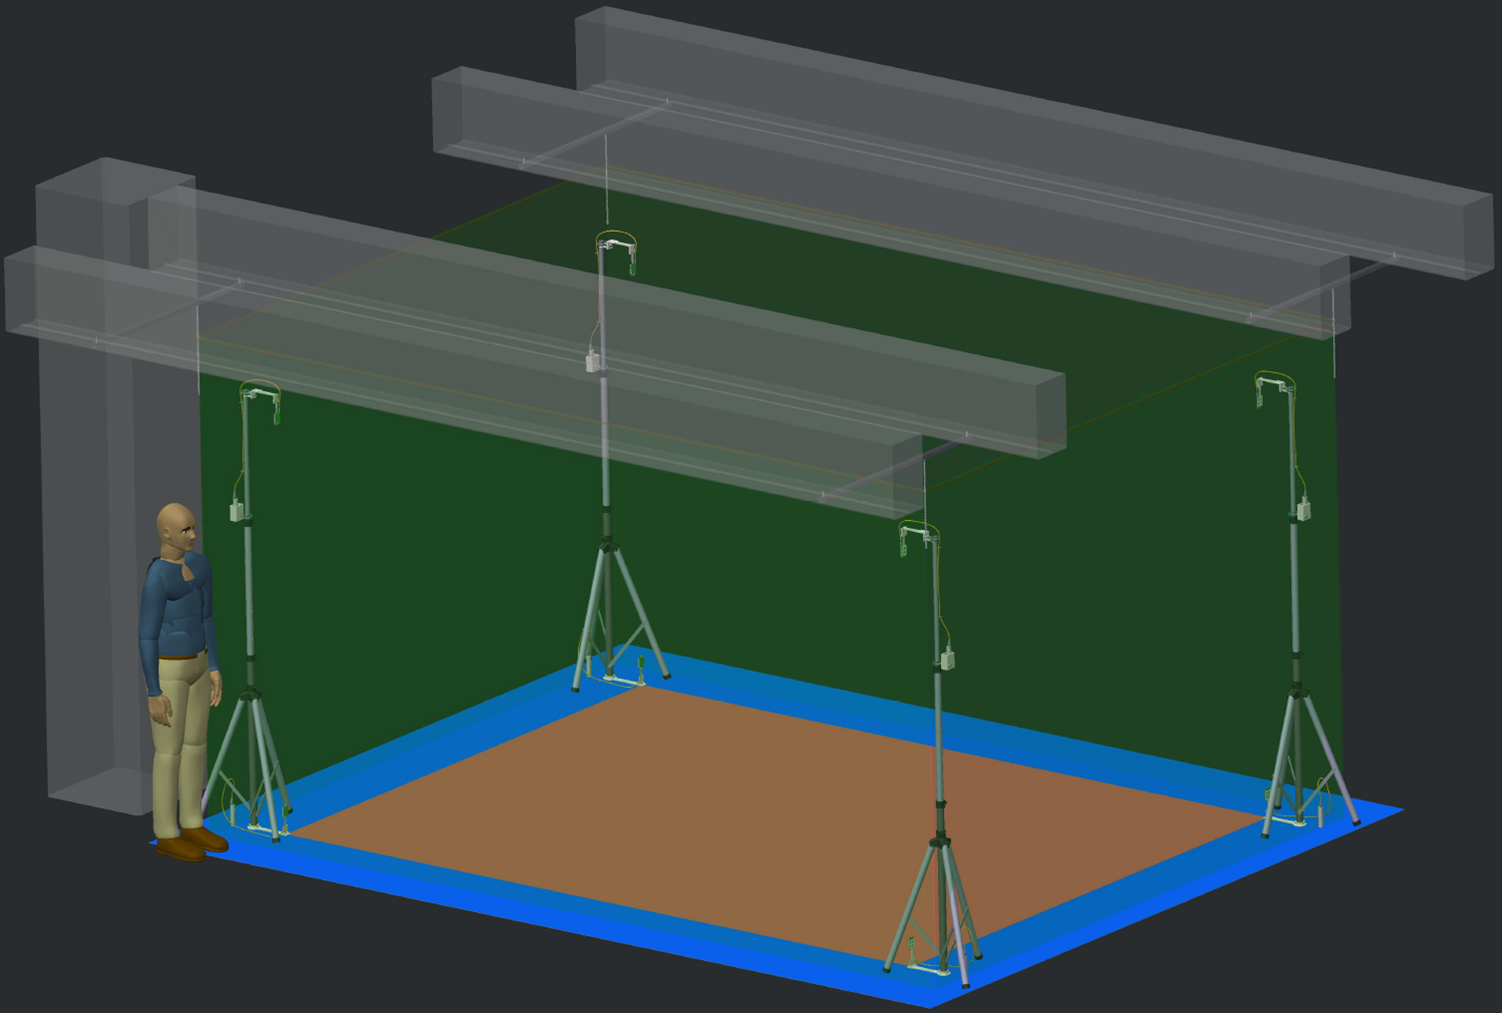
\includegraphics[width=6cm]{figures/LPS_Setup.png}
	\caption{LPS Setup}
	\label{fig:control_arch}	
\end{figure}		
\end{minipage}
	\hspace{0.05cm}
\begin{minipage}{0.35\textwidth}
    \begin{figure}[h!]
	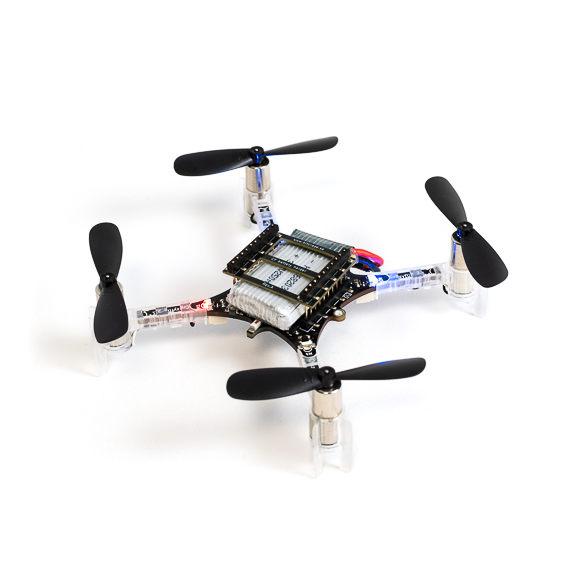
\includegraphics[width=4cm]{figures/crazyflie_2_1_585px.jpg}
	\caption{Crazyflie 2.1}
	\label{fig:control_arch}	
\end{figure}		
\end{minipage}

\begin{itemize}
	\item Indoor Positioning System called the Loco Position System (LPS) and Crazyflie 2.0 developed by the company bitcraze\footnote{https://www.bitcraze.io/products/crazyflie-2-1/}
	\item Implemented a peer-to-peer communication protocol \footnote{Paulsen, 2018.Master thesis.}
\end{itemize}
\end{frame}
%%%%%%%%%%%%%%%%%%%%%%%%%%%%%%%%%%%%%%%%%%%%%%%%%%%%%%%%%%%%%%%%%%%%%%
%\begin{frame}{Experimental results: Quadratic field}
%$\psi(q)=(q-c)^T\begin{bmatrix}1&0\\0&2\end{bmatrix}(q-c)$ with $c=\begin{bmatrix}2\\1.5\end{bmatrix}$
%\vspace{5cm}
%\end{frame}
%%%%%%%%%%%%%%%%%%%%%%%%%%%%%%%%%%%%%%%%%%%%%%%%%%%%%%%%%%%%%%%%%%%%%%
%\begin{frame}{Experimental results: Log-convex field}
%$\psi(q)=-\textnormal{exp}(-||q-c||^2)$ with $c=\begin{bmatrix}2\\1.5\end{bmatrix}$
%\vspace{5cm}	
%\end{frame}
%%%%%%%%%%%%%%%%%%%%%%%%%%%%%%%%%%%%%%%%%%%%%%%%%%%%%%%%%%%%%%%%%%%%%%
%\begin{frame}{Experimental results: Field with two minima}
%$\psi(q)=-\textnormal{exp}(-||q-c_1||^2)-\textnormal{exp}(-||q-c_2||^2)$ with $c_1=\begin{bmatrix}1\\1\end{bmatrix}$, $c_2=\begin{bmatrix}3\\2\end{bmatrix}$
%\vspace{5cm}	
%\end{frame}
%%%%%%%%%%%%%%%%%%%%%%%%%%%%%%%%%%%%%%%%%%%%%%%%%%%%%%%%%%%%%%%%%%%%%%
%\begin{frame}{Visualizing experimental results}
%
%\end{frame}
%%%%%%%%%%%%%%%%%%%%%%%%%%%%%%%%%%%%%%%%%%%%%%%%%%%%%%%%%%%%%%%%%%%%%
% \begin{frame}{Experimental results: Quadratic field}
% 	\textcolor{red}{Replace figure with animation and video} 
% 	\begin{figure}[h!]	
% 		\includegraphics[width=12cm]{figures/quadratic_field_contour.png}
% 		%\caption{Histograms of errors (in angles) between the estimated and true gradient direction and modified Newton step direction when the field measurements are corrupted}
% 		\label{fig:quadratic_field}
% 	\end{figure}
% \end{frame}
%%%%%%%%%%%%%%%%%%%%%%%%%%%%%%%%%%%%%%%%%%%%%%%%%%%%%%%%%%%%%%%%%%%%%
% \begin{frame}{Experimental results: Log-convex field}
% 	\textcolor{red}{Replace figure with animation and video}
% 	\begin{figure}[h!]	
% 		\includegraphics[width=12cm]{figures/log_convex_field_contour.png}
% 		%\caption{Histograms of errors (in angles) between the estimated and true gradient direction and modified Newton step direction when the field measurements are corrupted}
% 		\label{fig:log_convex_field}
% 	\end{figure}
% \end{frame}
%%%%%%%%%%%%%%%%%%%%%%%%%%%%%%%%%%%%%%%%%%%%%%%%%%%%%%%%%%%%%%%%%%%%%
% \begin{frame}{Experimental results: Non-convex field}
% 	\textcolor{red}{Replace figure with animation and video}
% 	\begin{figure}[h!]	
% 		\includegraphics[width=12cm]{figures/non_convex_field_contour.png}
% 		%\caption{Histograms of errors (in angles) between the estimated and true gradient direction and modified Newton step direction when the field measurements are corrupted}
% 		\label{fig:non_convex_field}
% 	\end{figure}
% \end{frame}
%%%%%%%%%%%%%%%%%%%%%%%%%%%%%%%%%%%%%%%%%%%%%%%%%%%%%%%%%%%%%%%%%%%%%%
% \begin{frame}{Experimental Results: Quadratic field(Video)}
% \includemedia[
% activate=pageopen,
% width=300pt,height=200pt,
% addresource=animations/OBLIQUE_quadratic_mod_newton_Fig_4.mp4,
% flashvars={%
% 	src=figures/noObstacle.mp4      % same path as in addresource!
% 	%&scaleMode=stretch % removes black bars
% 	&autoPlay=true      % optional configuration
% 	&loop=true          % variables
% }
% ]{}{StrobeMediaPlayback.swf}
% \end{frame}
% %%%%%%%%%%%%%%%%%%%%%%%%%%%%%%%%%%%%%%%%%%%%%%%%%%%%%%%%%%%%%%%%%%%%%%
% \begin{frame}{Experimental Results: Quadratic field(Animation)}

% 		\includemedia[
% 		activate=pageopen,
% 		width=300pt,height=200pt,
% 		addresource=animations/convex.mp4,
% 		flashvars={%
% 			src=figures/noObstacle.mp4      % same path as in addresource!
% 			%&scaleMode=stretch % removes black bars
% 			&autoPlay=true      % optional configuration
% 			&loop=true          % variables
% 		}
% 		]{}{StrobeMediaPlayback.swf}

% \end{frame}
% %%%%%%%%%%%%%%%%%%%%%%%%%%%%%%%%%%%%%%%%%%%%%%%%%%%%%%%%%%%%%%%%%%%%%%
% \begin{frame}{Experimental Results: Log-Convex quadratic field (Video)}
% 		\includemedia[
% 		activate=pagevisible,
% 		width=300pt,height=200pt,
% 		addresource=animations/OBLIQUEVIEW__log_convex_mod_newton_Fig_5.mp4,
% 		flashvars={%
% 			src=figures/noObstacle.mp4      % same path as in addresource!
% 			%&scaleMode=stretch % removes black bars
% 			&autoPlay=true      % optional configuration
% 			&loop=true          % variables
% 		}
% 		]{}{StrobeMediaPlayback.swf}
% \end{frame}
% %%%%%%%%%%%%%%%%%%%%%%%%%%%%%%%%%%%%%%%%%%%%%%%%%%%%%%%%%%%%%%%%%%%%%%
% \begin{frame}{Experimental Results: Log-Convex quadratic field (Animation)}
% 	\includemedia[
% 	activate=pagevisible,
% 	width=300pt,height=200pt,
% 	addresource=animations/quasiConvex.mp4,
% 	flashvars={%
% 		src=figures/noObstacle.mp4      % same path as in addresource!
% 		%&scaleMode=stretch % removes black bars
% 		&autoPlay=true      % optional configuration
% 		&loop=true          % variables
% 	}
% 	]{}{StrobeMediaPlayback.swf}
% \end{frame}
% %%%%%%%%%%%%%%%%%%%%%%%%%%%%%%%%%%%%%%%%%%%%%%%%%%%%%%%%%%%%%%%%%%%%%%
% \begin{frame}{Experimental Results: Field with multiple minima (Video)}
% 	\includemedia[
% 	activate=pageopen,
% 	width=300pt,height=200pt,
% 	addresource=animations/2 minima mod Newton noise.mp4,
% 	flashvars={%
% 		src=figures/noObstacle.mp4      % same path as in addresource!
% 		%&scaleMode=stretch % removes black bars
% 		&autoPlay=true      % optional configuration
% 		&loop=true          % variables
% 	}
% 	]{}{StrobeMediaPlayback.swf}
% \end{frame}
% %%%%%%%%%%%%%%%%%%%%%%%%%%%%%%%%%%%%%%%%%%%%%%%%%%%%%%%%%%%%%%%%%%%%%%
% \begin{frame}{Experimental Results: Field with multiple minima (Animation)}
% 	\includemedia[
% 	activate=pageopen,
% 	width=300pt,height=200pt,
% 	addresource=animations/2minima.mp4,
% 	flashvars={%
% 		src=figures/noObstacle.mp4      % same path as in addresource!
% 		%&scaleMode=stretch % removes black bars
% 		&autoPlay=true      % optional configuration
% 		&loop=true          % variables
% 	}
% 	]{}{StrobeMediaPlayback.swf}
% \end{frame}
%%%%%%%%%%%%%%%%%%%%%%%%%%%%%%%%%%%%%%%%%%%%%%%%%%%%%%%%%%%%%%%%%%%%%